\documentclass{article}

% Chinese Support using xeCJK
% \usepackage{xeCJK}
% \setCJKmainfont{SimSun}

% Chinese Support using CTeX
\usepackage{ctex}

% Math Support
\usepackage{amsmath}
\usepackage{amsfonts}
\usepackage{amssymb}
\usepackage{wasysym}
\newcommand{\angstrom}{\text{\normalfont\AA}}
\usepackage{fancyhdr}

% Graphics Support
\usepackage{graphicx}
\usepackage{float}

% Reduced page margin
\usepackage{geometry}
\geometry{a4paper,scale=0.8}

\usepackage{caption}
\usepackage{subcaption}

% d and e should be math operators
\newcommand*{\dif}{\mathop{}\!\mathrm{d}}
\newcommand*{\md}{\mathop{}\!\mathrm{d}}
\newcommand*{\me}{\mathrm{e}}

% No indent for each paragraph
% \usepackage{parskip}
% \setlength{\parindent}{0cm}

% Bold style for Greek letters
\usepackage{bm}
\let\Oldmathbf\mathbf
\renewcommand{\mathbf}[1]{\boldsymbol{\Oldmathbf{#1}}}

% More space for dfrac in cell
\usepackage{cellspace}
\setlength{\cellspacetoplimit}{5pt}
\setlength{\cellspacebottomlimit}{5pt}

% SI units
\newcommand{\si}[1]{\  \mathrm{#1}}

% Multi-line author information
\usepackage{authblk}
\author{物理(4+4)1801 \quad  胡喜平 \quad U201811966}
\affil{个人网站 https://hxp.plus/ \quad 电子邮件 hxp201406@gmail.com}

\title{近代物理实验预习笔记——双频外差激光干涉仪}

\pagestyle{fancy}
\fancyhf{}
\lhead{源码地址:https://github.com/hxp-plus/Notes/tree/master/Physics-Experiment}
\rfoot{第 \thepage 页}
\renewcommand{\headrulewidth}{1pt}
\renewcommand{\footrulewidth}{1pt}

\begin{document}

\maketitle\thispagestyle{fancy}

\section{实验内容}

\begin{itemize}
\item 使用声光调制器对激光光束进行调制,产生不同频率的激光。搭建\textbf{非偏振双频外差激光干涉仪}光路。
\item \textbf{不考虑偏振}的情况下,观察和比较参考光和测量光的干涉信号,通过两干涉信号相位差测量决定光程差,得出\textbf{相位差}与\textbf{反射镜移动位移}的函数关系。
\item 考虑偏振的情况下,设计\textbf{基于偏振的双频外差激光干涉仪},重复上述测量。
\end{itemize}

\section{实验原理和注意事项}

\subsection{非偏振双频激光干涉仪}

\textbf{非偏振双频激光干涉仪}如图所示,其中两束氦氖激光存在无论是到PD1还是PD2都存在一定的光程差,为了方便讨论将图上四个位置用字母A、B、C、D表示。PD表示光电测量器,AOM表示声光调制器。

\begin{figure}[H]
  \centering
  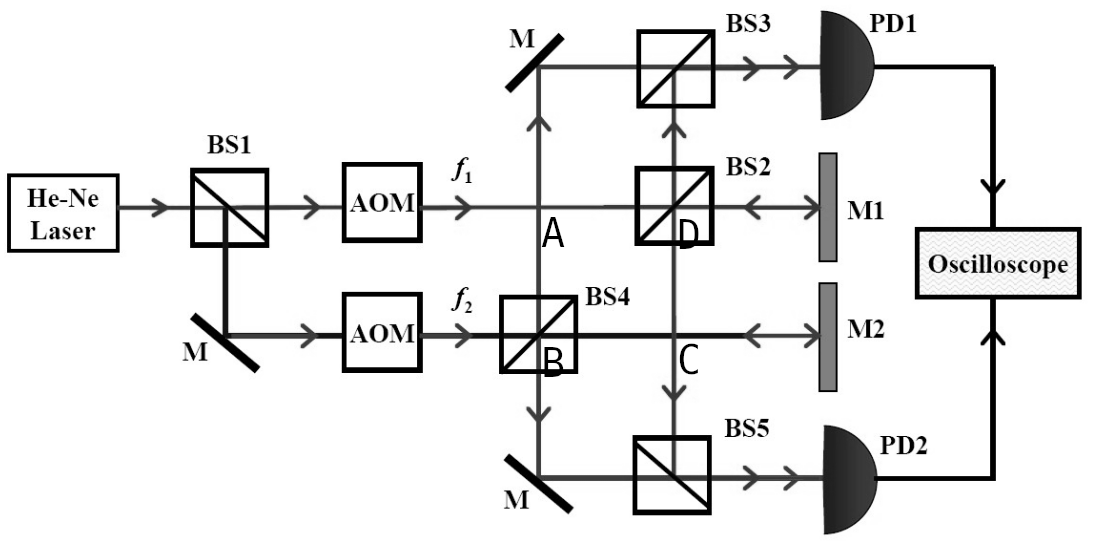
\includegraphics[width=0.9\linewidth]{figures/非偏振双频激光干涉仪}
  \caption{非偏振双频激光干涉仪示意图}
\end{figure}

其中抵达PD1的是参考光,抵达PD2的是测量光。实验中直接测量的量是两组干涉激光的测量信号的相位差$\Delta \phi$,间接测量反射镜M2与M1的相对位移$\Delta L$。

我们假设刚开始两个反射镜水平方向是没有位移的,那么对于\textbf{参考光},频率为$f_2$的光比频率为$f_1$的光多走的距离是$2 \overline{AB}$。而对于\textbf{测量光},频率为$f_2$的光比频率为$f_1$的光多走的距离是$2 \overline{BC}$。

因此为了防止出现奇怪的情况,在搭建实验光路的时候,应当使得\textbf{矩形ABCD}是\textbf{正方形}。其中实验中测量到的信号的光强信号为:

\begin{itemize}
\item 参考光:$I_r \propto I_0 \cos \left[ 2 \pi \left( f_1 - f_2 \right)t + \left( \varphi_{01} - \varphi_{02} \right) \right] $
\item 测量光:$I_m \propto I_0 \cos \left[ 2 \pi \left( f_1 - f_2 \right)t + \left( \varphi_{01} - \varphi_{02} \right) + \Delta \phi \right] $
\end{itemize}

两个反射镜之间的相对位移为:

\begin{equation*}
  \begin{aligned}
    \Delta L = \dfrac{\lambda}{4 \pi} \Delta \phi 
  \end{aligned}
\end{equation*}

\subsection{偏振双频激光干涉仪}

下面是一个\textbf{偏振双频激光干涉仪}示例

\begin{figure}[H]
  \centering
  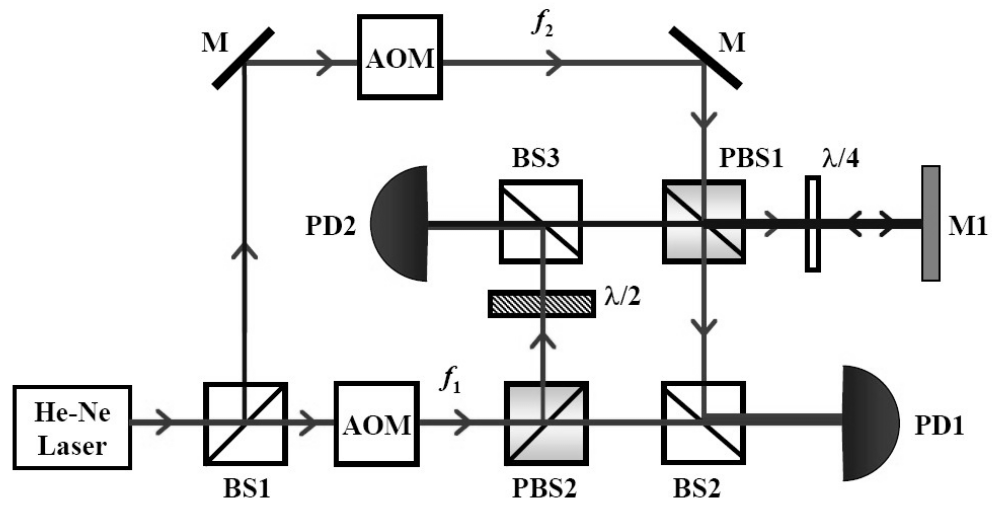
\includegraphics[width=0.9\linewidth]{figures/偏振双频激光干涉仪}
  \caption{偏振双频激光干涉仪示意图}
\end{figure}

通过移动反射镜M1,造成测量光的相位发生变化,由于M1到PBS1的距离光走一来一回了两遍,反射镜位移和相位差之间的关系依然是:

\begin{equation*}
  \begin{aligned}
    \Delta L = \dfrac{\lambda}{4 \pi} \Delta \phi
  \end{aligned}
\end{equation*}

因此用示波器测量$\Delta \phi$可以间接测量$\Delta L$。

\end{document} 
